
% LaTeX Beamer file automatically generated from DocOnce
% https://github.com/doconce/doconce

%-------------------- begin beamer-specific preamble ----------------------

\documentclass{beamer}

\usetheme{red_plain}
\usecolortheme{default}

% turn off the almost invisible, yet disturbing, navigation symbols:
\setbeamertemplate{navigation symbols}{}

% Examples on customization:
%\usecolortheme[named=RawSienna]{structure}
%\usetheme[height=7mm]{Rochester}
%\setbeamerfont{frametitle}{family=\rmfamily,shape=\itshape}
%\setbeamertemplate{items}[ball]
%\setbeamertemplate{blocks}[rounded][shadow=true]
%\useoutertheme{infolines}
%
%\usefonttheme{}
%\useinntertheme{}
%
%\setbeameroption{show notes}
%\setbeameroption{show notes on second screen=right}

% fine for B/W printing:
%\usecolortheme{seahorse}

\usepackage{pgf}
\usepackage{graphicx}
\usepackage{epsfig}
\usepackage{relsize}

\usepackage{fancybox}  % make sure fancybox is loaded before fancyvrb

\usepackage{fancyvrb}
%\usepackage{minted} % requires pygments and latex -shell-escape filename
%\usepackage{anslistings}
%\usepackage{listingsutf8}

\usepackage{amsmath,amssymb,bm}
%\usepackage[latin1]{inputenc}
\usepackage[T1]{fontenc}
\usepackage[utf8]{inputenc}
\usepackage{colortbl}
\usepackage[english]{babel}
\usepackage{tikz}
\usepackage{framed}
% Use some nice templates
\beamertemplatetransparentcovereddynamic

% --- begin table of contents based on sections ---
% Delete this, if you do not want the table of contents to pop up at
% the beginning of each section:
% (Only section headings can enter the table of contents in Beamer
% slides generated from DocOnce source, while subsections are used
% for the title in ordinary slides.)
\AtBeginSection[]
{
  \begin{frame}<beamer>[plain]
  \frametitle{}
  %\frametitle{Outline}
  \tableofcontents[currentsection]
  \end{frame}
}
% --- end table of contents based on sections ---

% If you wish to uncover everything in a step-wise fashion, uncomment
% the following command:

%\beamerdefaultoverlayspecification{<+->}

\newcommand{\shortinlinecomment}[3]{\note{\textbf{#1}: #2}}
\newcommand{\longinlinecomment}[3]{\shortinlinecomment{#1}{#2}{#3}}

\definecolor{linkcolor}{rgb}{0,0,0.4}
\hypersetup{
    colorlinks=true,
    linkcolor=linkcolor,
    urlcolor=linkcolor,
    pdfmenubar=true,
    pdftoolbar=true,
    bookmarksdepth=3
    }
\setlength{\parskip}{0pt}  % {1em}

\newenvironment{doconceexercise}{}{}
\newcounter{doconceexercisecounter}
\newenvironment{doconce:movie}{}{}
\newcounter{doconce:movie:counter}

\newcommand{\subex}[1]{\noindent\textbf{#1}}  % for subexercises: a), b), etc

%-------------------- end beamer-specific preamble ----------------------

% Add user's preamble




% insert custom LaTeX commands...

\raggedbottom
\makeindex

%-------------------- end preamble ----------------------

\begin{document}

% matching end for #ifdef PREAMBLE

\newcommand{\exercisesection}[1]{\subsection*{#1}}



% ------------------- main content ----------------------



% ----------------- title -------------------------

\title{Kvanteteknologi og kunstig intelligens}

% ----------------- author(s) -------------------------

\author{Morten Hjorth-Jensen\inst{1}}
\institute{Department of Physics and Center for Computing in Science Education, University of Oslo, Norway\inst{1}}
% ----------------- end author(s) -------------------------

\date{Faglig pedagogisk dag, 31 2024
% <optional titlepage figure>
% <optional copyright>
}

\begin{frame}[plain,fragile]
\titlepage
\end{frame}

\begin{frame}[plain,fragile]
\frametitle{Kort oppsumering}

\begin{block}{}
Kvanteteknologi og kunstig intelligens er teknologier som vil kunne
revolusjonere måten vi jobber og lever på og er forventa å kunne gi
store fordeler for vitenskapelig og teknologisk utvikling, og vil
sannsynligvis påvirke store og/eller alle deler av framtidas samfunn.
Foredraget her vil ta for seg hvordan disse teknologiene vil påvirke
naturfaglig og teknologisk forskning og undervisning, og hvorfor det
er så viktig å forstå mulighetene og begrensningene.
\end{block}

\begin{block}{}
Lysark finner du her  \href{{https://github.com/mhjensenseminars/MachineLearningTalk/tree/master/doc/pub/FPD}}{\nolinkurl{https://github.com/mhjensenseminars/MachineLearningTalk/tree/master/doc/pub/FPD}}
\end{block}
\end{frame}

\begin{frame}[plain,fragile]
\frametitle{AI/ML and some statements you may have heard (and what do they mean?)}

https://www.businessenergyuk.com/knowledge-hub/chatgpt-energy-consumption-visualized/



\begin{enumerate}
\item Fei-Fei Li on ImageNet: \textbf{map out the entire world of objects} (\href{{https://cacm.acm.org/news/219702-the-data-that-transformed-ai-research-and-possibly-the-world/fulltext}}{The data that transformed AI research})

\item Russell and Norvig in their popular textbook: \textbf{relevant to any intellectual task; it is truly a universal field} (\href{{http://aima.cs.berkeley.edu/}}{Artificial Intelligence, A modern approach})

\item Woody Bledsoe puts it more bluntly: \textbf{in the long run, AI is the only science} (quoted in Pamilla McCorduck, \href{{https://www.pamelamccorduck.com/machines-who-think}}{Machines who think})
\end{enumerate}

\noindent
If you wish to have a critical read on AI/ML from a societal point of view, see \href{{https://www.katecrawford.net/}}{Kate Crawford's recent text Atlas of AI}.

\textbf{Here: with AI/ML we intend a collection of machine learning methods with an emphasis on statistical learning and data analysis}
\end{frame}

\begin{frame}[plain,fragile]
\frametitle{Curse of dimensionality}

\vspace{6mm}

% inline figure
\centerline{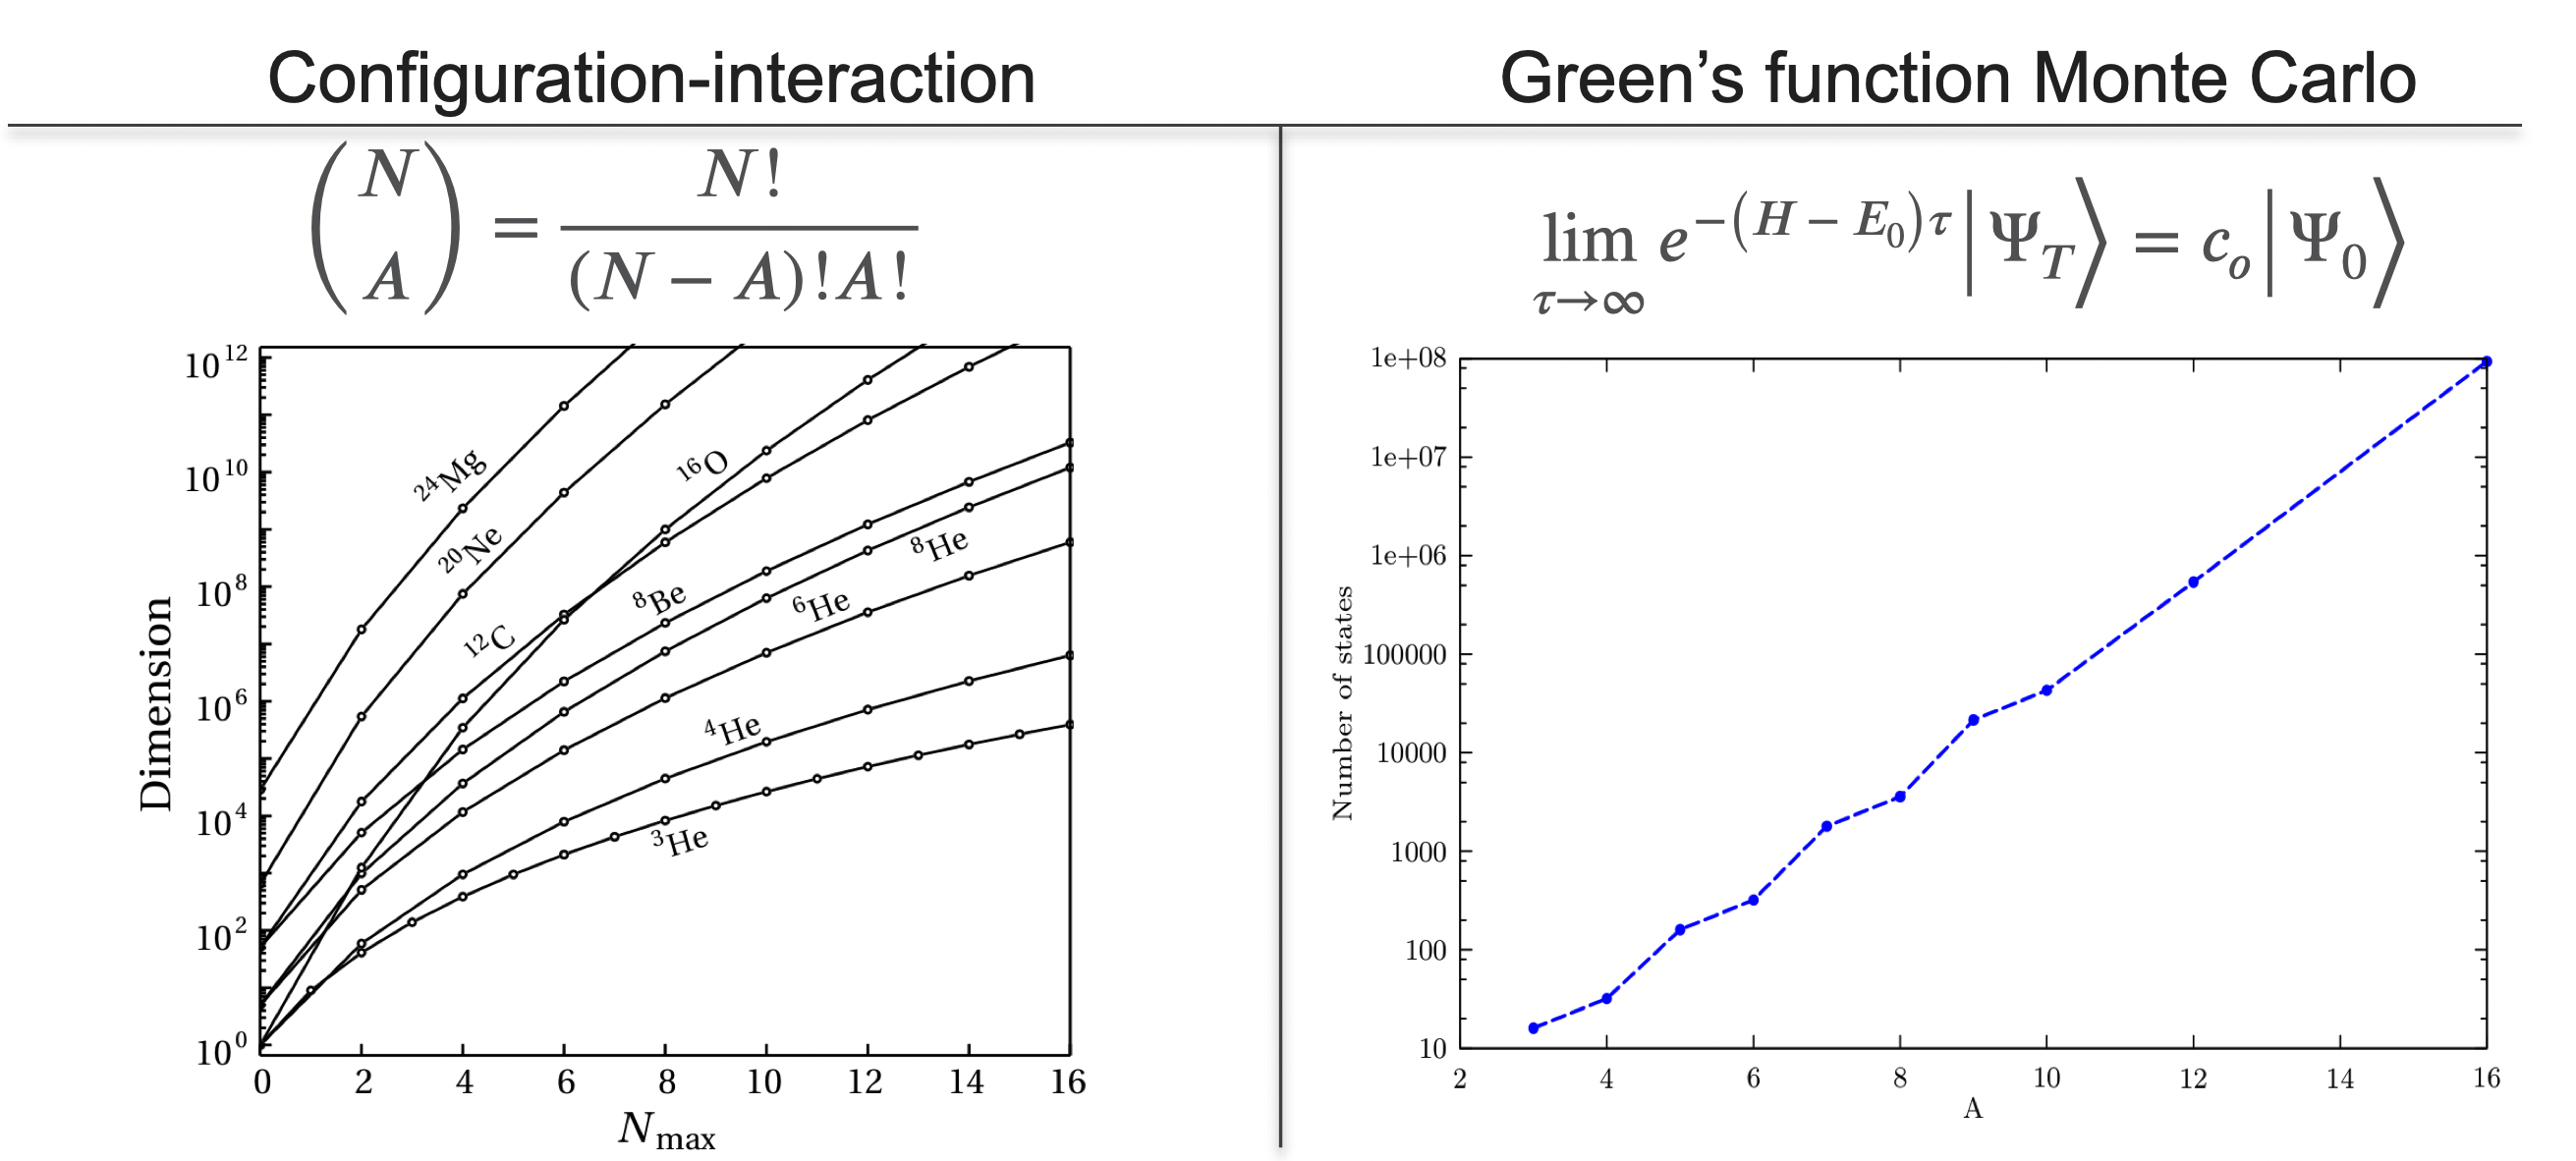
\includegraphics[width=1.0\linewidth]{figures/mbpfig2.png}}

\vspace{6mm}
\end{frame}

\begin{frame}[plain,fragile]
\frametitle{Neural network quantum states}

\begin{block}{Neural networks compactly represent complex high-dimensional functions }
Most quantum states of interest have distinctive features and intrinsic structures
%FIGURE: [figures/mbpfig3.png, width=900 frac=1.0]
\end{block}
\end{frame}

\begin{frame}[plain,fragile]
\frametitle{Machine learning. A simple perspective on the interface between ML and Physics}

\vspace{6mm}

% inline figure
\centerline{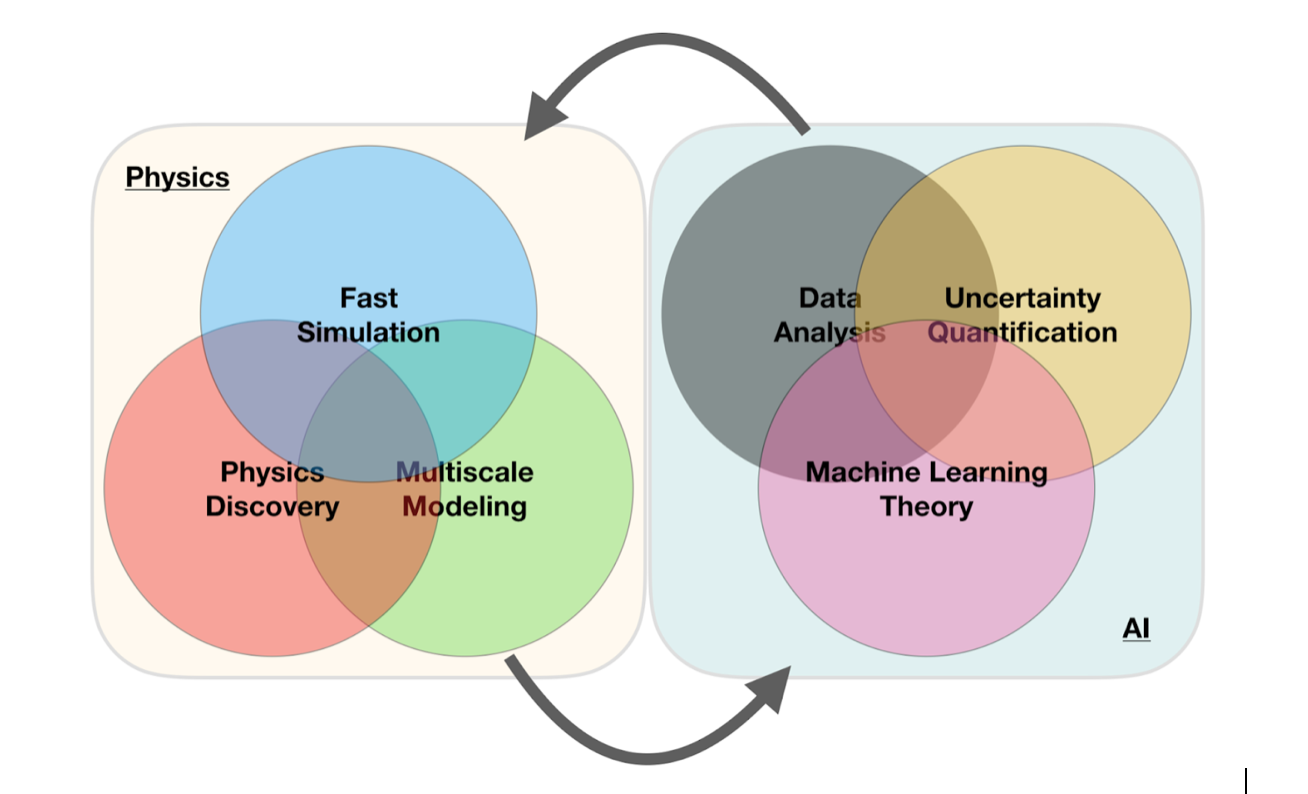
\includegraphics[width=1.0\linewidth]{figures/mlimage.png}}

\vspace{6mm}
\end{frame}

\begin{frame}[plain,fragile]
\frametitle{Types of machine learning}

\begin{block}{}
The approaches to machine learning are many, but are often split into two main categories. 
In \emph{supervised learning} we know the answer to a problem,
and let the computer deduce the logic behind it. On the other hand, \emph{unsupervised learning}
is a method for finding patterns and relationship in data sets without any prior knowledge of the system.

An important  third category is  \emph{reinforcement learning}. This is a paradigm 
of learning inspired by behavioural psychology, where learning is achieved by trial-and-error, 
solely from rewards and punishment.
\end{block}
\end{frame}

\begin{frame}[plain,fragile]
\frametitle{Main categories}

\begin{block}{}
Another way to categorize machine learning tasks is to consider the desired output of a system.
Some of the most common tasks are:

\begin{itemize}
  \item Classification: Outputs are divided into two or more classes. The goal is to   produce a model that assigns inputs into one of these classes. An example is to identify  digits based on pictures of hand-written ones. Classification is typically supervised learning.

  \item Regression: Finding a functional relationship between an input data set and a reference data set.   The goal is to construct a function that maps input data to continuous output values.

  \item Clustering: Data are divided into groups with certain common traits, without knowing the different groups beforehand.  It is thus a form of unsupervised learning.
\end{itemize}

\noindent
\end{block}
\end{frame}

\begin{frame}[plain,fragile]
\frametitle{The plethora  of machine learning algorithms/methods}

\begin{enumerate}
\item Deep learning: Neural Networks (NN), Convolutional NN, Recurrent NN, Boltzmann machines, autoencoders and variational autoencoders  and generative adversarial networks, stable diffusion and many more generative models

\item Bayesian statistics and Bayesian Machine Learning, Bayesian experimental design, Bayesian Regression models, Bayesian neural networks, Gaussian processes and much more

\item Dimensionality reduction (Principal component analysis), Clustering Methods and more

\item Ensemble Methods, Random forests, bagging and voting methods, gradient boosting approaches 

\item Linear and logistic regression, Kernel methods, support vector machines and more

\item Reinforcement Learning; Transfer Learning and more 
\end{enumerate}

\noindent
\end{frame}

\begin{frame}[plain,fragile]
\frametitle{Example of discriminative modeling, \href{{https://www.oreilly.com/library/view/generative-deep-learning/9781098134174/ch01.html}}{taken from Generative Deep Learning by David Foster}}

\vspace{6mm}

% inline figure
\centerline{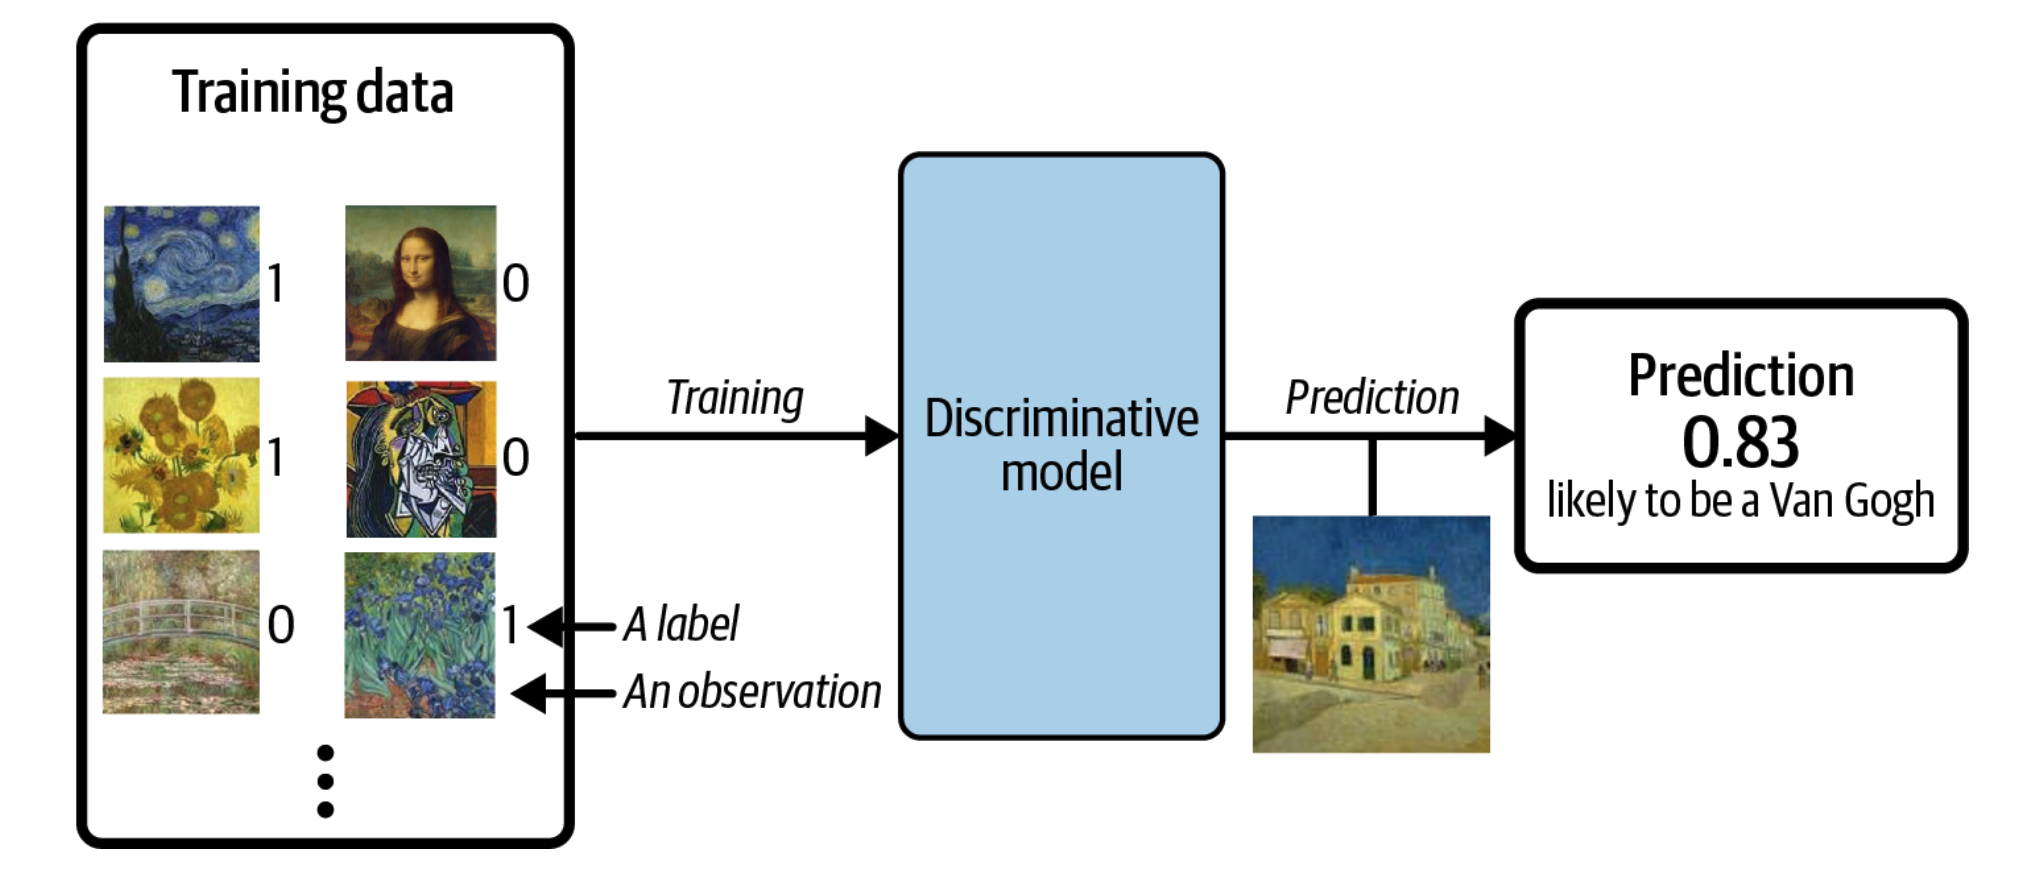
\includegraphics[width=1.0\linewidth]{figures/standarddeeplearning.png}}

\vspace{6mm}
\end{frame}

\begin{frame}[plain,fragile]
\frametitle{Example of generative modeling, \href{{https://www.oreilly.com/library/view/generative-deep-learning/9781098134174/ch01.html}}{taken from Generative Deep Learning by David Foster}}

\vspace{6mm}

% inline figure
\centerline{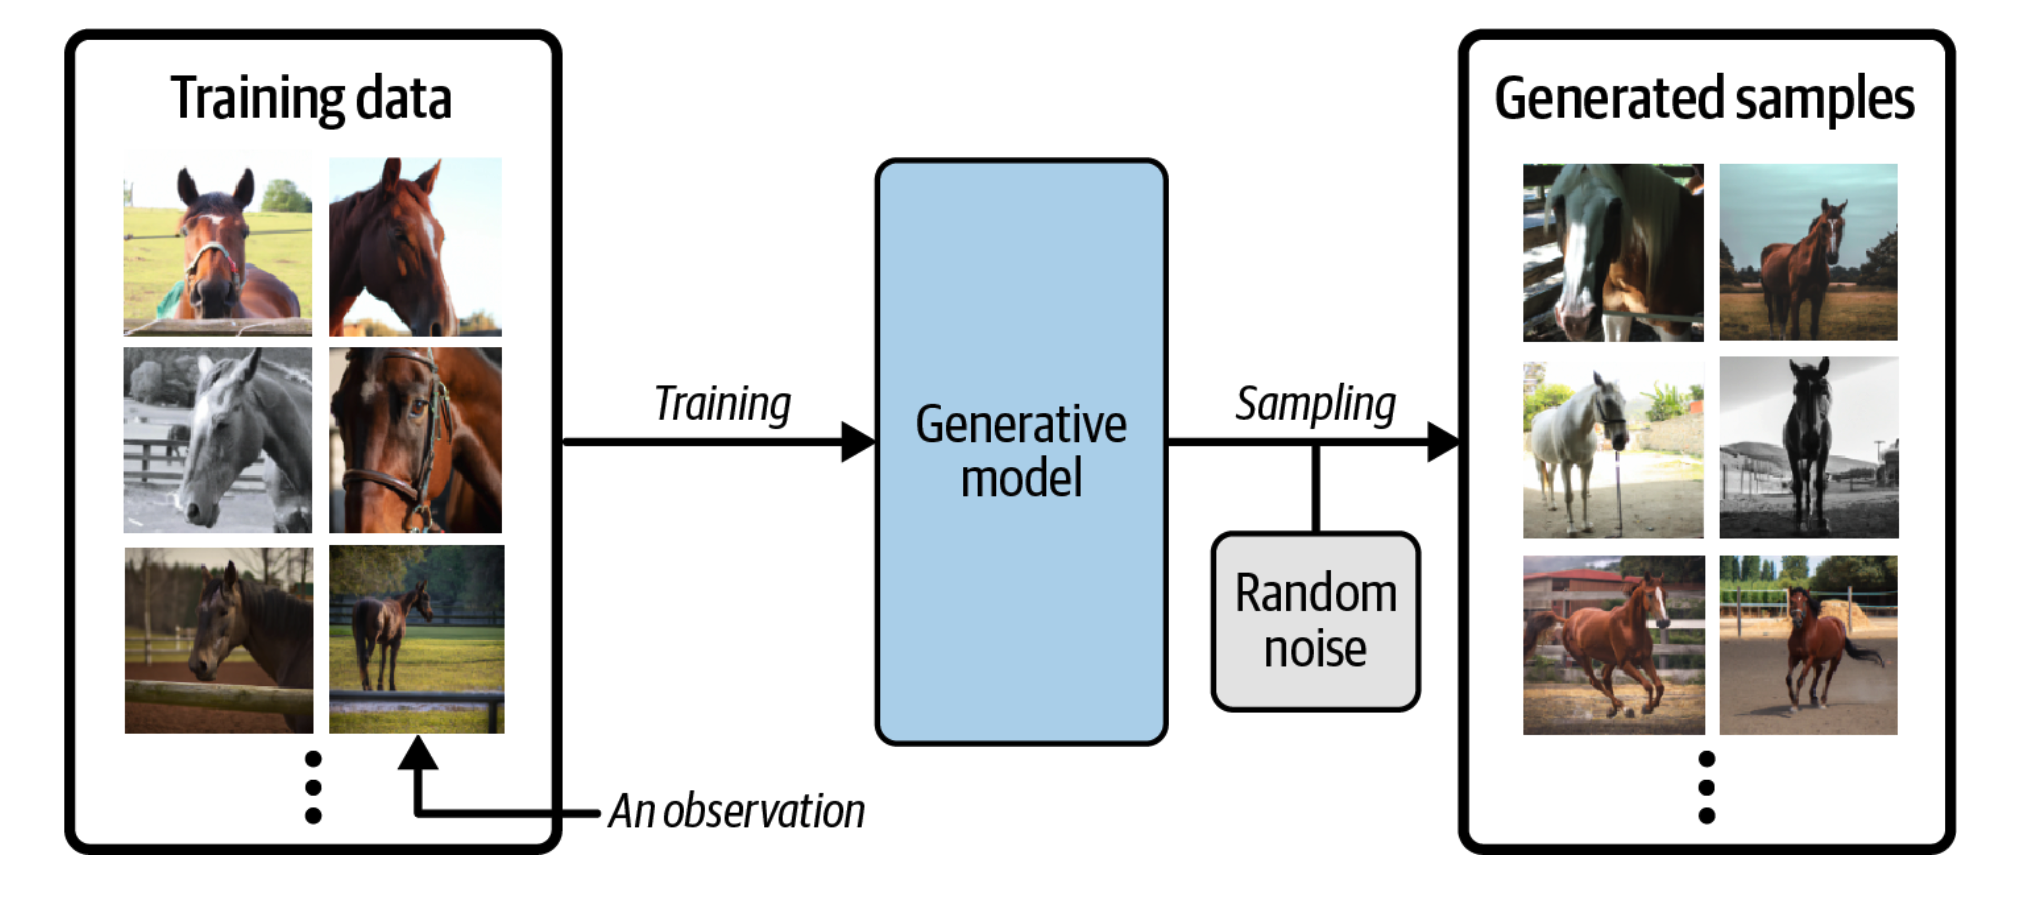
\includegraphics[width=1.0\linewidth]{figures/generativelearning.png}}

\vspace{6mm}
\end{frame}

\begin{frame}[plain,fragile]
\frametitle{Taxonomy of generative deep learning, \href{{https://www.oreilly.com/library/view/generative-deep-learning/9781098134174/ch01.html}}{taken from Generative Deep Learning by David Foster}}

\vspace{6mm}

% inline figure
\centerline{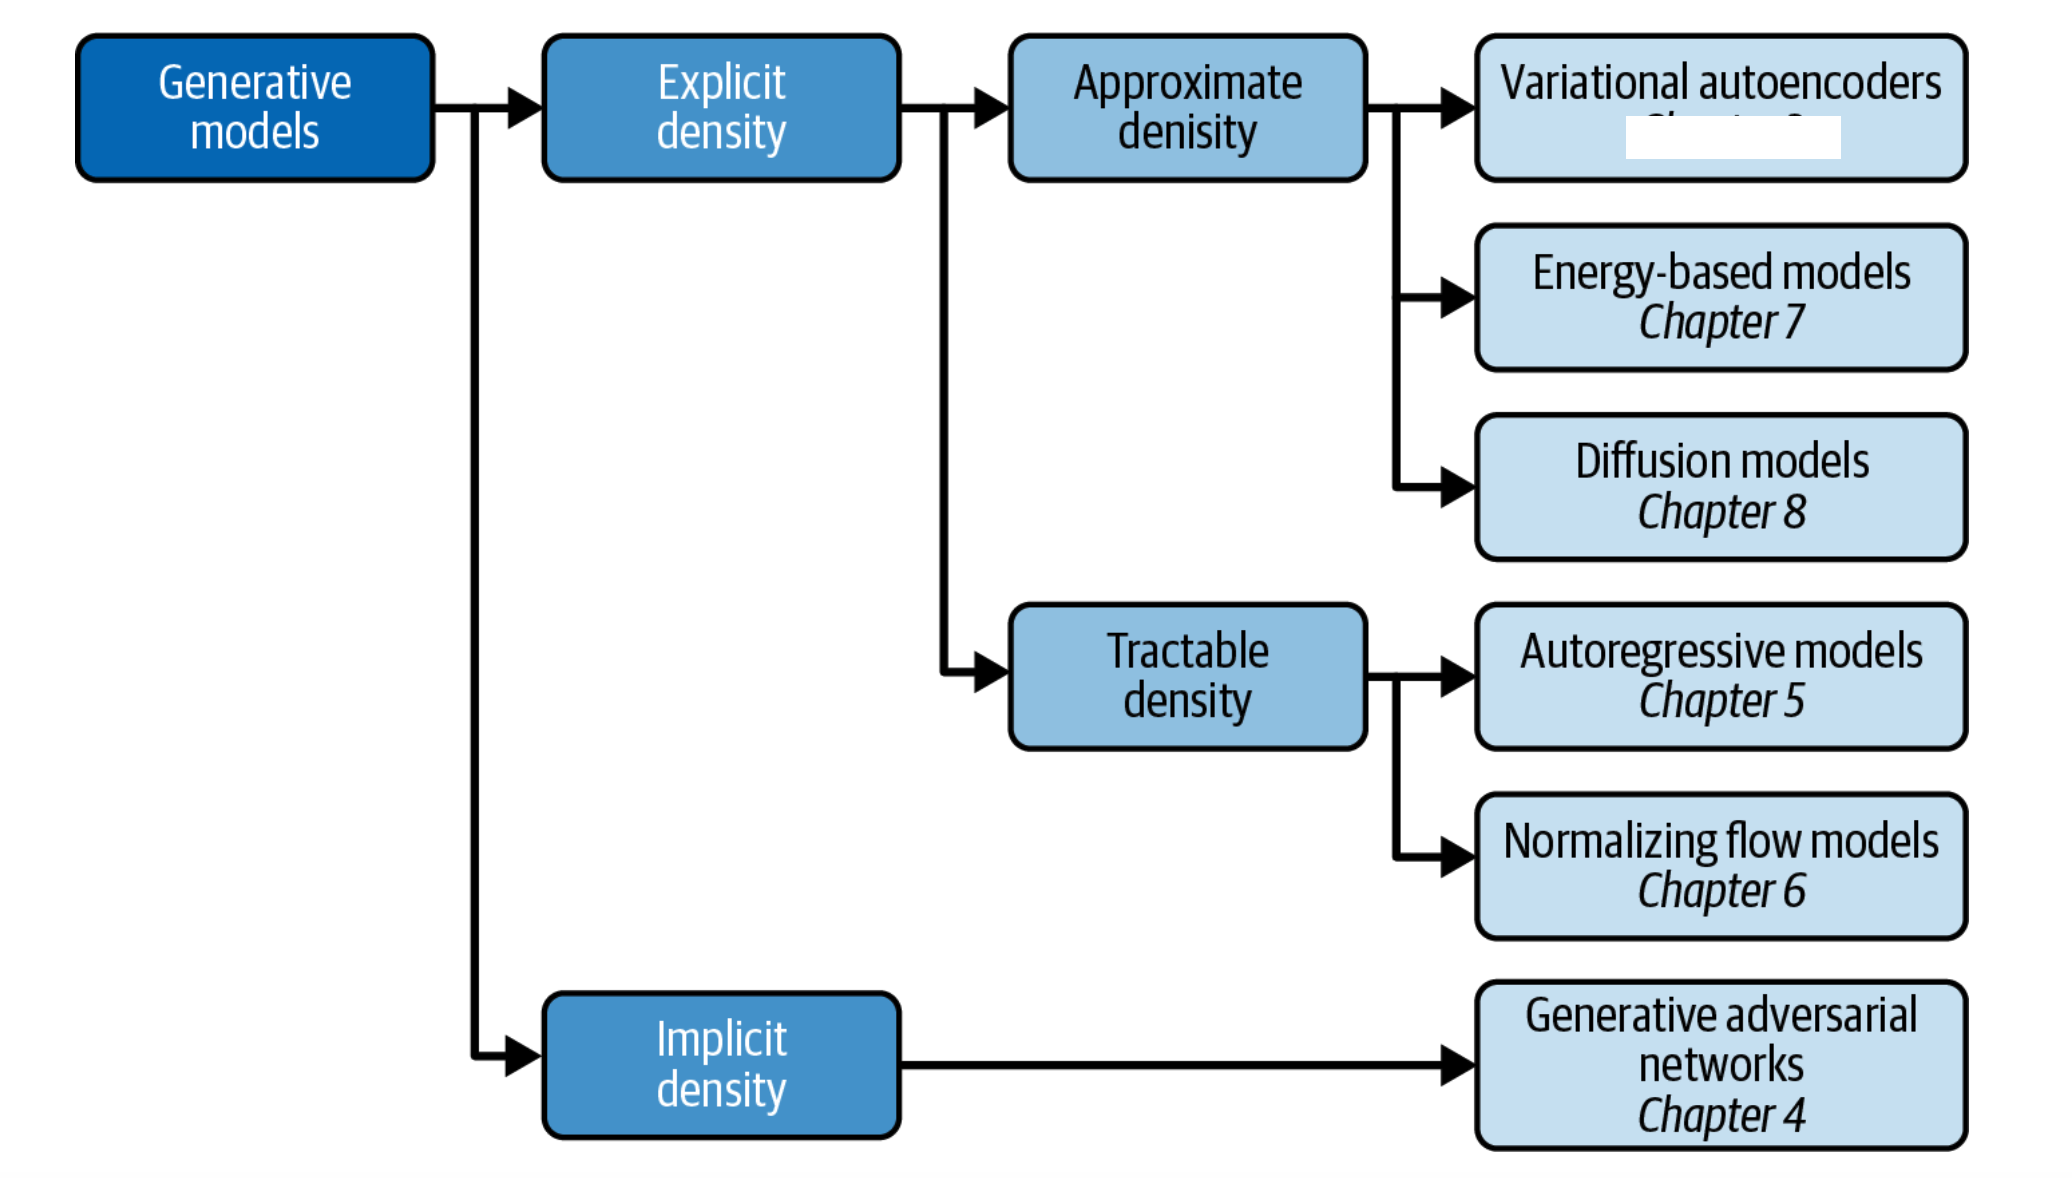
\includegraphics[width=1.0\linewidth]{figures/generativemodels.png}}

\vspace{6mm}
\end{frame}

\begin{frame}[plain,fragile]
\frametitle{Good books with hands-on material and codes}

\begin{block}{}
\begin{itemize}
\item \href{{https://sebastianraschka.com/blog/2022/ml-pytorch-book.html}}{Sebastian Rashcka et al, Machine learning with Sickit-Learn and PyTorch}

\item \href{{https://www.oreilly.com/library/view/generative-deep-learning/9781098134174/ch01.html}}{David Foster, Generative Deep Learning with TensorFlow}

\item \href{{https://github.com/PacktPublishing/Hands-On-Generative-AI-with-Python-and-TensorFlow-2}}{Babcock and Gavras, Generative AI with Python and TensorFlow 2}
\end{itemize}

\noindent
\end{block}

All three books have GitHub sites from where  one can download all codes. A good and more general text (2016)
is Goodfellow, Bengio and Courville, \href{{https://www.deeplearningbook.org/}}{Deep Learning}
\end{frame}

\begin{frame}[plain,fragile]
\frametitle{More references}

\begin{block}{Reading on diffusion models }
\begin{enumerate}
\item A central paper is the one by Sohl-Dickstein et al, Deep Unsupervised Learning using Nonequilibrium Thermodynamics, \href{{https://arxiv.org/abs/1503.03585}}{\nolinkurl{https://arxiv.org/abs/1503.03585}}

\item See also Diederik P. Kingma, Tim Salimans, Ben Poole, Jonathan Ho, Variational Diffusion Models, \href{{https://arxiv.org/abs/2107.00630}}{\nolinkurl{https://arxiv.org/abs/2107.00630}}
\end{enumerate}

\noindent
\end{block}   

\begin{block}{and VAEs }
\begin{enumerate}
\item An Introduction to Variational Autoencoders, by Kingma and Welling, see \href{{https://arxiv.org/abs/1906.02691}}{\nolinkurl{https://arxiv.org/abs/1906.02691}}
\end{enumerate}

\noindent
\end{block}

\textbf{And two Nobel prizes this year. Physics and Chemistry}
\end{frame}

\begin{frame}[plain,fragile]
\frametitle{What are the basic Machine Learning ingredients?}

\begin{block}{}
Almost every problem in ML and data science starts with the same ingredients:
\begin{itemize}
\item The dataset $\bm{x}$ (could be some observable quantity of the system we are studying)

\item A model which is a function of a set of parameters $\bm{\alpha}$ that relates to the dataset, say a likelihood  function $p(\bm{x}\vert \bm{\alpha})$ or just a simple model $f(\bm{\alpha})$

\item A so-called \textbf{loss/cost/risk} function $\mathcal{C} (\bm{x}, f(\bm{\alpha}))$ which allows us to decide how well our model represents the dataset. 
\end{itemize}

\noindent
We seek to minimize the function $\mathcal{C} (\bm{x}, f(\bm{\alpha}))$ by finding the parameter values which minimize $\mathcal{C}$. This leads to  various minimization algorithms. It may surprise many, but at the heart of all machine learning algortihms there is an optimization problem. 
\end{block}
\end{frame}

\begin{frame}[plain,fragile]
\frametitle{Low-level machine learning, the family of ordinary least squares methods}

Our data which we want to apply a machine learning method on, consist
of a set of inputs $\bm{x}^T=[x_0,x_1,x_2,\dots,x_{n-1}]$ and the
outputs we want to model $\bm{y}^T=[y_0,y_1,y_2,\dots,y_{n-1}]$.
We assume  that the output data can be represented (for a regression case) by a continuous function $f$
through
\[
\bm{y}=f(\bm{x})+\bm{\epsilon}.
\]
\end{frame}

\begin{frame}[plain,fragile]
\frametitle{Setting up the equations}

In linear regression we approximate the unknown function with another
continuous function $\tilde{\bm{y}}(\bm{x})$ which depends linearly on
some unknown parameters
$\bm{\theta}^T=[\theta_0,\theta_1,\theta_2,\dots,\theta_{p-1}]$.

The input data can be organized in terms of a so-called design matrix 
with an approximating function $\bm{\tilde{y}}$ 
\[
\bm{\tilde{y}}= \bm{X}\bm{\theta},
\]
\end{frame}

\begin{frame}[plain,fragile]
\frametitle{The objective/cost/loss function}

The  simplest approach is the mean squared error
\[
C(\bm{\Theta})=\frac{1}{n}\sum_{i=0}^{n-1}\left(y_i-\tilde{y}_i\right)^2=\frac{1}{n}\left\{\left(\bm{y}-\bm{\tilde{y}}\right)^T\left(\bm{y}-\bm{\tilde{y}}\right)\right\},
\]
or using the matrix $\bm{X}$ and in a more compact matrix-vector notation as
\[
C(\bm{\Theta})=\frac{1}{n}\left\{\left(\bm{y}-\bm{X}\bm{\theta}\right)^T\left(\bm{y}-\bm{X}\bm{\theta}\right)\right\}.
\]
This function represents one of many possible ways to define the so-called cost function.
\end{frame}

\begin{frame}[plain,fragile]
\frametitle{Training solution}

Optimizing with respect to the unknown parameters $\theta_j$ we get 
\[
\bm{X}^T\bm{y} = \bm{X}^T\bm{X}\bm{\theta},  
\]
and if the matrix $\bm{X}^T\bm{X}$ is invertible we have the optimal values
\[
\hat{\bm{\theta}} =\left(\bm{X}^T\bm{X}\right)^{-1}\bm{X}^T\bm{y}.
\]

We say we 'learn' the unknown parameters $\bm{\theta}$ from the last equation.
\end{frame}

\begin{frame}[plain,fragile]
\frametitle{Selected references}

\begin{block}{}
\begin{itemize}
\item \href{{https://arxiv.org/abs/1803.08823}}{Mehta et al.} and \href{{https://www.sciencedirect.com/science/article/pii/S0370157319300766?via%3Dihub}}{Physics Reports (2019)}.

\item \href{{https://link.aps.org/doi/10.1103/RevModPhys.91.045002}}{Machine Learning and the Physical Sciences by Carleo et al}

\item \href{{https://journals.aps.org/rmp/abstract/10.1103/RevModPhys.94.031003}}{Artificial Intelligence and Machine Learning in Nuclear Physics, Amber Boehnlein et al., Reviews Modern of Physics 94, 031003 (2022)} 

\item \href{{https://pdg.lbl.gov/2021/reviews/rpp2021-rev-machine-learning.pdf}}{Particle Data Group summary on ML methods}
\end{itemize}

\noindent
\end{block}
\end{frame}

\begin{frame}[plain,fragile]
\frametitle{Scientific Machine Learning}

An important and emerging field is what has been dubbed as scientific ML, see the article by Deiana et al, Applications and Techniques for Fast Machine Learning in Science, Big Data \textbf{5}, 787421 (2022) \href{{https://doi.org/10.3389/fdata.2022.787421}}{\nolinkurl{https://doi.org/10.3389/fdata.2022.787421}}

\begin{block}{}
The authors discuss applications and techniques for fast machine
learning (ML) in science -- the concept of integrating power ML
methods into the real-time experimental data processing loop to
accelerate scientific discovery. The report covers three main areas

\begin{enumerate}
\item applications for fast ML across a number of scientific domains;

\item techniques for training and implementing performant and resource-efficient ML algorithms;

\item and computing architectures, platforms, and technologies for deploying these algorithms.
\end{enumerate}

\noindent
\end{block}
\end{frame}

\begin{frame}[plain,fragile]
\frametitle{ML for detectors}

\vspace{6mm}

% inline figure
\centerline{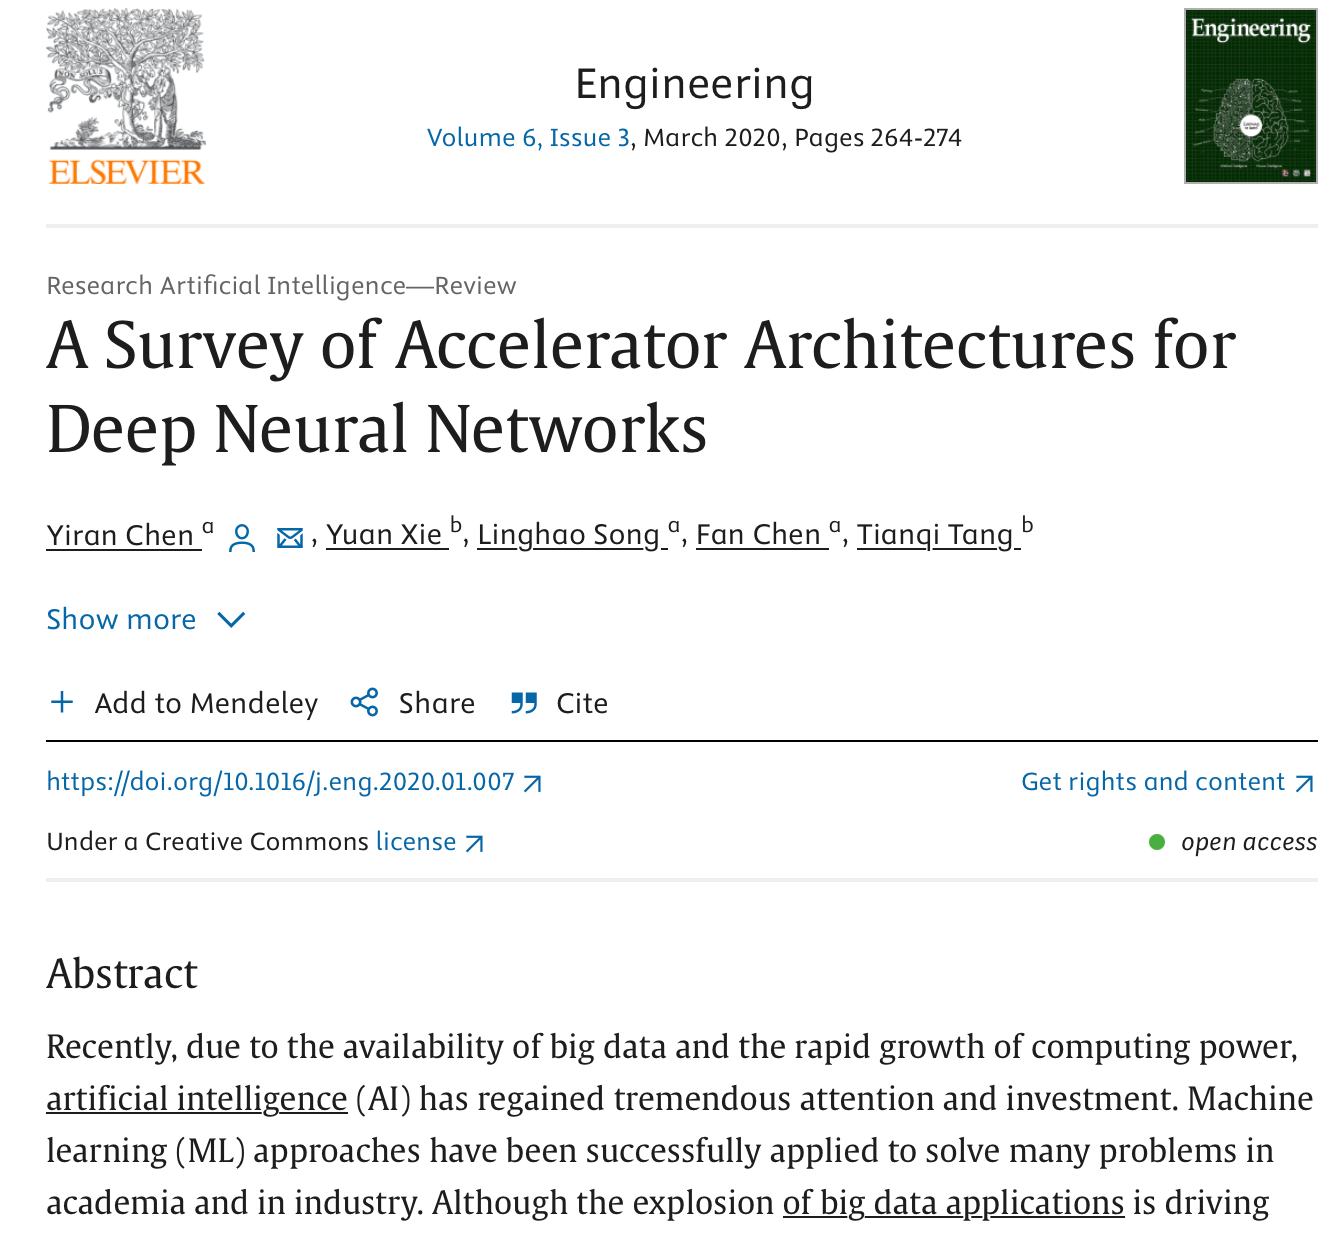
\includegraphics[width=1.0\linewidth]{figures/detectors.png}}

\vspace{6mm}
\end{frame}

\begin{frame}[plain,fragile]
\frametitle{Physics driven Machine Learning}

Another hot topic is what has loosely been dubbed \textbf{Physics-driven deep learning}. See the recent work on \href{{https://www.nature.com/articles/s42256-021-00302-5}}{Learning nonlinear operators via DeepONet based on the universal approximation theorem of operators, Nature Machine Learning, vol 3, 218 (2021)}.

\begin{block}{From their abstract }
A less known but powerful result is that an NN with a single hidden layer can accurately approximate any nonlinear continuous operator. This universal approximation theorem of operators is suggestive of the structure and potential of deep neural networks (DNNs) in learning continuous operators or complex systems from streams of scattered data. ...  We demonstrate that DeepONet can learn various explicit operators, such as integrals and fractional Laplacians, as well as implicit operators that represent deterministic and stochastic differential equations. 
\end{block}
\end{frame}

\begin{frame}[plain,fragile]
\frametitle{Argon-46 by Solli et al., NIMA 1010, 165461 (2021)}

\begin{block}{}
Representations of two events from the
Argon-46 experiment. Each row is one event in two projections,
where the color intensity of each point indicates higher charge values
recorded by the detector. The bottom row illustrates a carbon event with
a large fraction of noise, while the top row shows a proton event
almost free of noise. 
\end{block}

\vspace{6mm}

% inline figure
\centerline{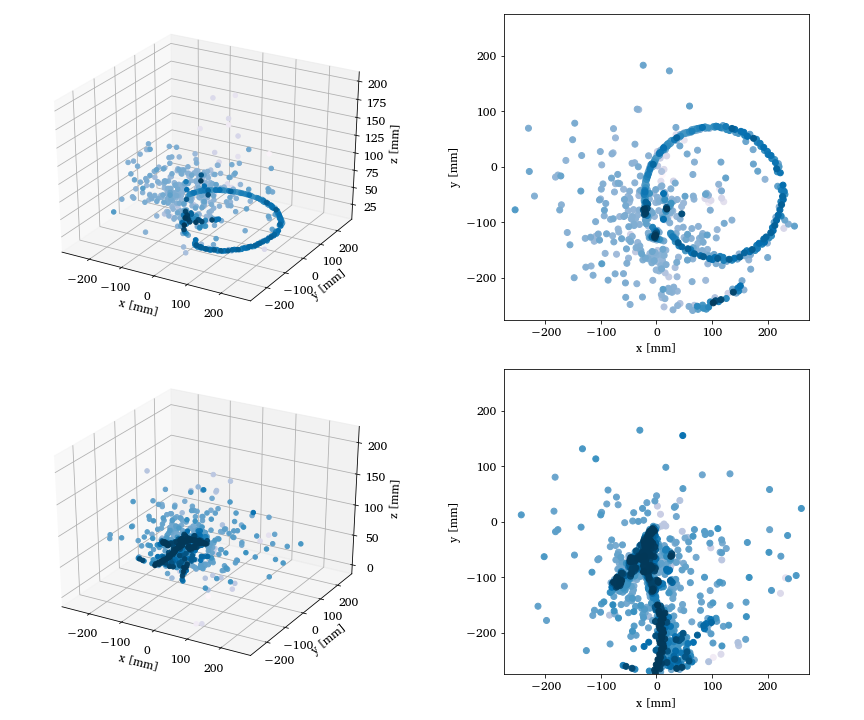
\includegraphics[width=0.6\linewidth]{figures/examples_raw.png}}

\vspace{6mm}
\end{frame}

\begin{frame}[plain,fragile]
\frametitle{Neutron star structure}

\vspace{6mm}

% inline figure
\centerline{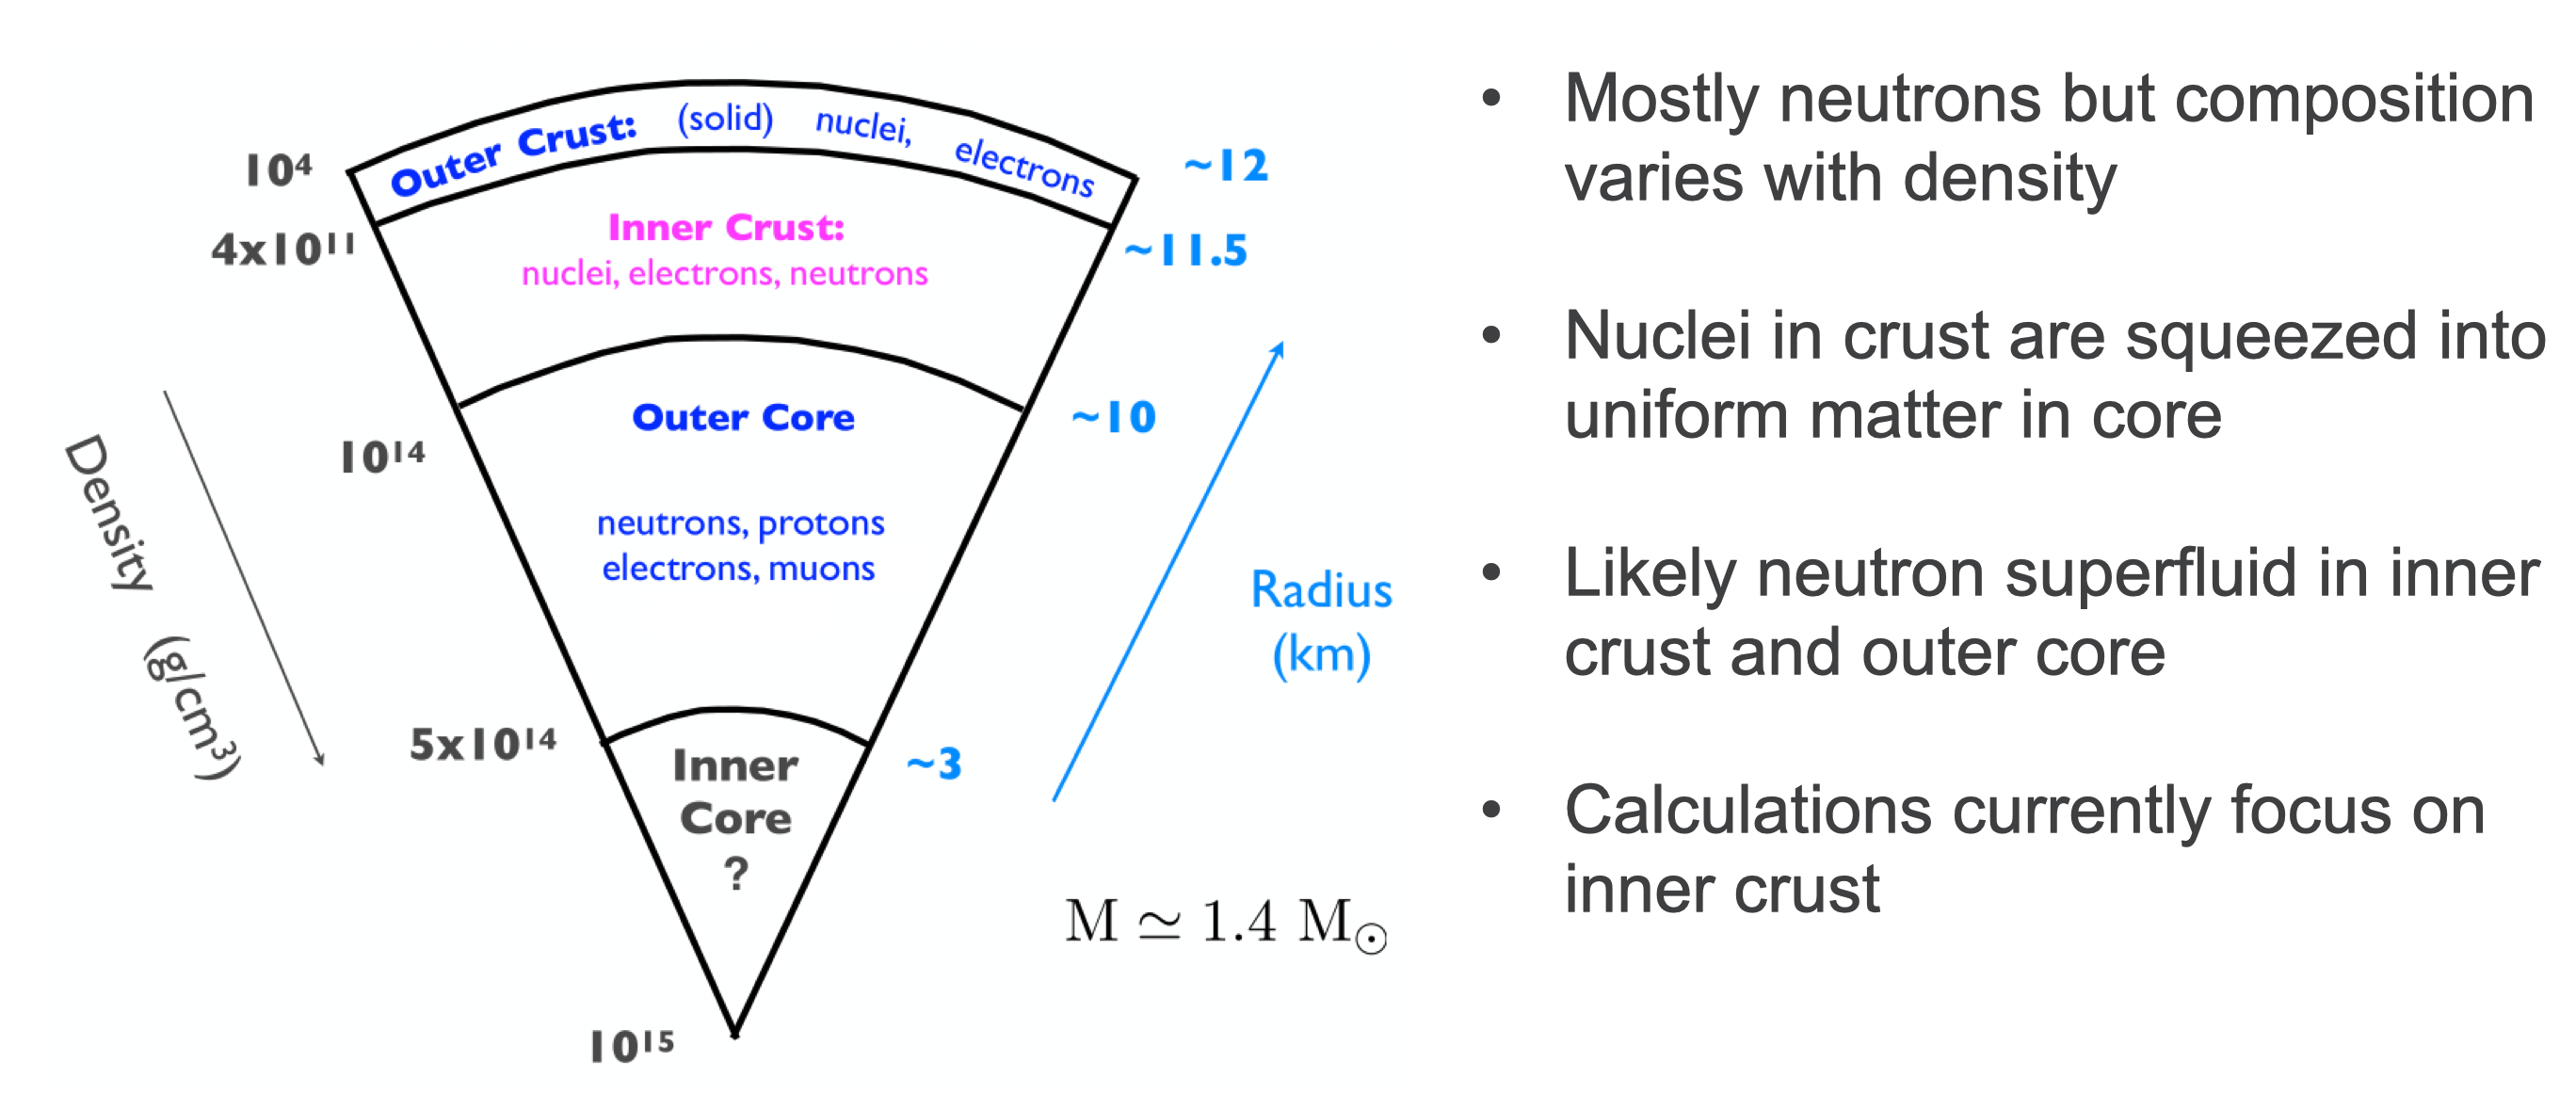
\includegraphics[width=1.0\linewidth]{figures/mbpfig5.png}}

\vspace{6mm}
\end{frame}

\begin{frame}[plain,fragile]
\frametitle{\href{{https://journals.aps.org/prresearch/pdf/10.1103/PhysRevResearch.5.033062}}{Dilute neutron star matter from neural-network quantum states by Fore et al, Physical Review Research 5, 033062 (2023)} at density $\rho=0.04$ fm$^{-3}$}

\begin{block}{}

\vspace{6mm}

% inline figure
\centerline{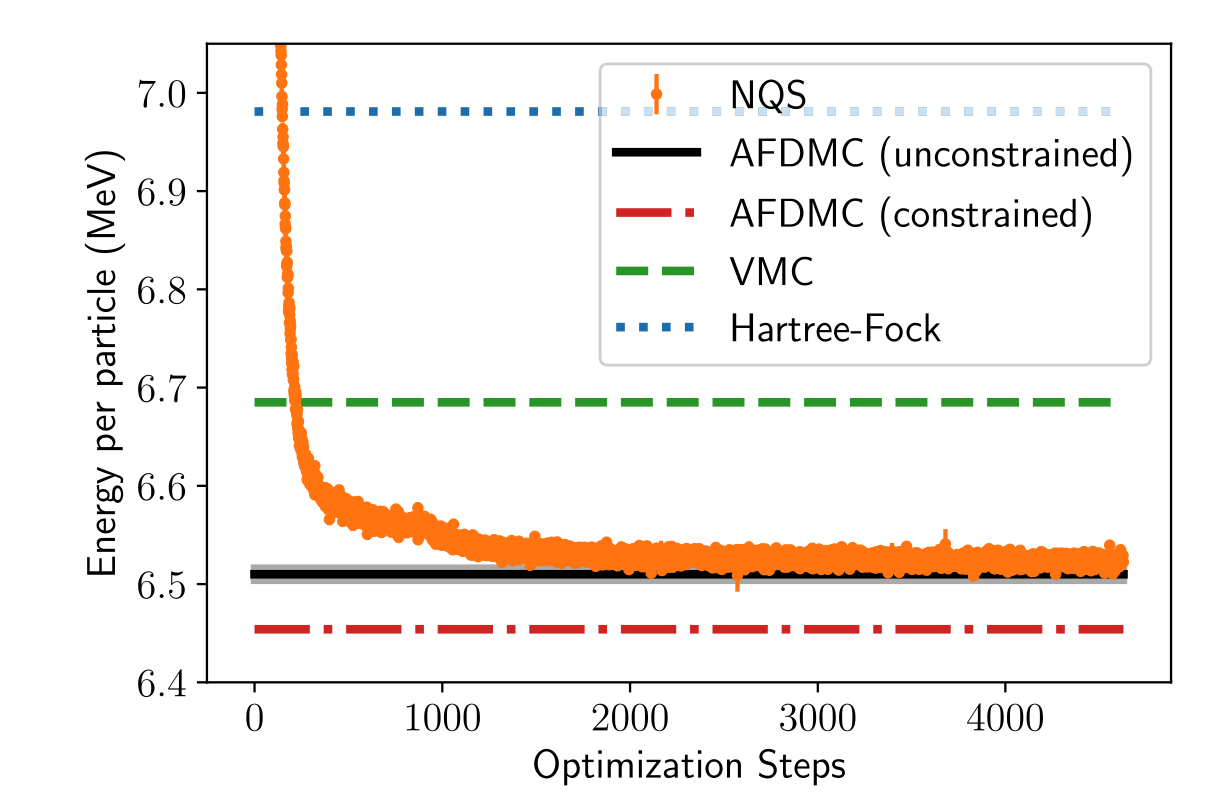
\includegraphics[width=0.9\linewidth]{figures/nmatter.png}}

\vspace{6mm}

\end{block}
\end{frame}

\begin{frame}[plain,fragile]
\frametitle{Education and advanced training}

\begin{block}{}
\begin{enumerate}
\item Outreach and communication on quantum technologies and AI, explaining quantum technologies and AI to a broader audience

\item Research on education in AI and QT. How are these topics best communicated and implemented in different enviroments, from  high school education to universities and to a broader audience, including external partners

\item QAI-TALENT, Education and knowledge transfer through the development of advanced educational programs
\end{enumerate}

\noindent
\end{block}
\end{frame}

\begin{frame}[plain,fragile]
\frametitle{Education, Quantum and AI/Machine Learning}

At the university of Oslo we have now established several educational
programs in AI and QTs and quantum science. These programs span the
whole spectrum from beginners courses to advanced training and
education tailored to the specific needs of the participants.

Furthermore, through research done at the center for Computing in
Science Education and the physics education research group at the
department of physics of the university of Oslo, we have over the
years developed knowledge and insights on how to teach central
concepts in quantum science as well as developing computational
literacy and understanding of central algorithms applied to scientific
problems.
\end{frame}

\begin{frame}[plain,fragile]
\frametitle{Courses and study programs}

\begin{enumerate}
\item \textbf{New study direction on Quantum technology} in Bachelor program Physics and Astronomy, starts Fall 2024. Three new courses:
\begin{itemize}

  \item FYS1400 Introduction to Quantum Technologies

  \item FYS3405/4405 Quantum Materials

  \item FYS3415/4415 Quantum Computing

\end{itemize}

\noindent
\item \textbf{Developed Master of Science program on Computational Science}, started fall  2018 and many students here work on quantum computing and machine learning

\item Developed courses on machine learning, from basic to advanced ones

\item Developed advanced course on quantum computing and quantum machine learning, MAT3420, MAT4430/9430, FYS5419/9419

\item New study directions in Master of Science in Physics and Computational Science on Quantum technologies and more. Start fall 2025
\end{enumerate}

\noindent
\end{frame}

\begin{frame}[plain,fragile]
\frametitle{Content of courses we offer}

\begin{block}{}
\begin{enumerate}
\item Quantum Information theory

\item From Classical Information theory to Quantum Information theory

\item Classical and Quantum Laboratory 

\item Discipline-Based Quantum Mechanics 

\item Quantum algorithms, computing, software and hardware

\item Several  machine learning/AI courses, at all levels
\end{enumerate}

\noindent
\end{block}
\end{frame}

\begin{frame}[plain,fragile]
\frametitle{QAI-TALENT: Education for a broader audience}

We have yearslong experience (with research based evidence on what works or not) in developing intensive training courses on ML/AI and QT.
We  plan to develop an educational activity on quantum science and AI, \textbf{QAI TALENT}
(TALENT=Training and Advanced Lectures in EmergiNg Technologies) offering

\begin{block}{}
\begin{enumerate}
\item Intensive short courses on selected topics (which can lead to credits and certificates)

\item Certificates of expertise with modules that can add up to one year of credits or more.

\item Possibilities of adding up to a master specialization in quantum science/technologies and/or AI/ML

\item Common educational projects and supervision of students
\end{enumerate}

\noindent
\end{block}
\end{frame}

\begin{frame}[plain,fragile]
\frametitle{Research directions, not exhaustive}

\begin{block}{}
\begin{enumerate}
\item \textbf{Theory and experiments for quantum sensors}, from standard many-body theories, via machine learning to quantum computing. Close collaboration with Norwegian industry

\item \textbf{Theory and experiments for quantum computing and quantum information theory}

\item \textbf{Fundamental studies (theory and experiment) of quantum mechanics}
\end{enumerate}

\noindent
\end{block}
\end{frame}

\end{document}
